%
% preprint.tex
%
\documentclass[a4paper, 12pt]{article}

\usepackage[14pt]{extsizes}

\usepackage{amsmath, amssymb, mathtools}
\usepackage{amsthm}
\usepackage{cmap}
\usepackage{rotating}
\usepackage{framed}

\usepackage[utf8]{inputenc}
\usepackage[english,russian]{babel}
\usepackage[pdftex,unicode]{hyperref}
\usepackage[left=2cm,right=2cm,top=2cm,bottom=3cm,bindingoffset=0cm]{geometry}
\usepackage{indentfirst}

\usepackage{subcaption}

\usepackage{todonotes}

\usepackage{ccaption}
% заменяем для рисунков ‘:’ после номера рисунка на ‘.’
\captiondelim{. }
\usepackage[labelsep=period]{caption}

\usepackage{mdframed}


% %%%%%%%%%%%%%%%%%%%%%%%%%%%%%%%%%%%%%%%%%%%%%%%%%%%%%%%%%%%%%%%%%%%%%%%%%%%%%%%
% Показать метки
% \usepackage{showkeys}[draft]
%\usepackage{showkeys}[final]

% %%%%%%%%%%%%%%%%%%%%%%%%%%%%%%%%%%%%%%%%%%%%%%%%%%%%%%%%%%%%%%%%%%%%%%%%%%%%%%%
%
\newcommand{\te}{\text{E}}
\newcommand{\txtr}{\text{r}}
\newcommand{\tj}{\text{J}}
\newcommand{\tem}{\text{EM}}
\newcommand{\tint}{\text{INT}}





% ---
% Commands and operators
\newcommand{\tpr}{\boldsymbol{\otimes}}   % tensor product
\newcommand{\dpr}{\boldsymbol{\cdot}}     % dot product
\newcommand{\cpr}{\boldsymbol{\times}}    % cross product
\newcommand{\sm}{\boldsymbol{:}}          % оператор свертки TODO: Сделать его оператором!


\newcommand{\tn}[1]{\boldsymbol{#1}}      % bold for tensor values
\newcommand{\vc}[1]{\boldsymbol{#1}}      % bold for vector values

\newcommand{\rclr}[1]{{\color{red} #1}}
\newcommand{\tnt}{{\tn{T}}}      % bold for tensor T

\newcommand{\vcx}{{\vc{x}}}      % bold for vector x
\newcommand{\vcn}{{\vc{n}}}      % bold for vector n
\newcommand{\vce}{{\vc{e}}}      % bold for vector e

\newcommand{\vct}{{\vc{t}}}      % bold for vector t
\newcommand{\vcu}{{\vc{u}}}      % bold for vector u
\newcommand{\vcv}{{\vc{v}}}      % bold for vector u
\newcommand{\vcw}{{\vc{w}}}      % bold for vector u


% %%%%%%%%%%%%%%%%%%%%%%%%%%%%%%%%%%%%%%%%%%%%%%%%%%%%%%%%%%%%%%%%%%%%%%%%%%%%%%%%%%%%%%%%%%%%%%%%%%%
% Commands
\newcommand{\mcS}{{\mathcal{S}}}
\newcommand{\mcF}{{\mathcal{F}}}
\newcommand{\pmcF}{{\partial\mathcal{F}}}
\newcommand{\mcI}{{\mathcal{I}}}

\newcommand{\mc}[1]{{\mathcal{#1}}}



\DeclareMathOperator{\codim} {codim}
\DeclareMathOperator{\dist}{{dist}}
\DeclareMathOperator{\argmin}{{arg\,min}}
\DeclareMathOperator{\sgnd}{{sign\,dist}}
\DeclareMathOperator{\sign}{sign}
\DeclareMathOperator{\tr}{tr}
\DeclareMathOperator{\diam}{diam}
\DeclareMathOperator{\diag}{diag}
\DeclareMathOperator{\dv}{div}
\DeclareMathOperator{\grd}{grad}
\DeclareMathOperator{\supp}{{supp}}

\newcommand{\dhudhx}[2]{\frac{\partial_h{#1}}{\partial_h{#2}}}

\newcommand{\dudx}[2]{\frac{\partial{#1}}{\partial{#2}}}
\newcommand{\dudxf}[2]{\frac{d{#1}}{d{#2}}}
\newcommand{\ddudx}[2]{\cfrac{\partial^2{#1}}{\partial{#2}^2}}
\newcommand{\ddudxy}[3]{\cfrac{\partial^2{#1}}{\partial{#2}\partial{#3}}}
\newcommand{\dvv}[1]{\dv\left(#1\right)}
%\newcommand{\grad}[1]{\grd\left(#1\right)}
\newcommand{\grad}[1]{\nabla\left(#1\right)}

\newcommand{\sqr}[1]{\left(#1\right)^{\!2}}

\def\onedot{$\mathsurround0pt\ldotp$}
\def\cddot{% two dots stacked vertically
  \mathbin{\vcenter{\baselineskip.67ex
      \hbox{\onedot}\hbox{\onedot}}%
        }}%

%\newcommand{\vec}[1]{\mathbf #1}

\newcommand{\la}{\langle}
\newcommand{\ra}{\rangle}

\newcommand{\mmm}{\text{м}$^3$}

\newcommand{\unitPa}{\text{Па}}
\newcommand{\unitSec}{\text{с}}
\newcommand{\unitM}{\text{м}}
\newcommand{\unitKg}{\text{кг}}
\newcommand{\unitK}{\text{К}}
\newcommand{\unitJ}{\text{Дж}}
\newcommand{\unitMole}{\text{моль}}
\newcommand{\unitDarcy}{\text{Дарси}}

% Жирное начертание для некоторых латинских букв в формулах
% Жирным начертанием обозначаются вектора
\newcommand{\bX}{ {\boldsymbol{x}}  }
\newcommand{\bx}{ {\boldsymbol{x}}  }
\newcommand{\bM}{ {\boldsymbol{M}}  }
\newcommand{\bF}{ {\boldsymbol{F}}  }
\newcommand{\bJ}{ {\boldsymbol{J}}  }
\newcommand{\prt}{ {\partial}  }

% Безразмерные величины -- величины с тильдами
\newcommand{\rtd}{\widetilde{\rho}}
\newcommand{\ptd}{\widetilde{p}}
\newcommand{\etd}{\widetilde{e}}
\newcommand{\Etd}{\widetilde{E}}
\newcommand{\Htd}{\widetilde{H}}
\newcommand{\ttd}{\widetilde{t}}
\newcommand{\xtd}{\widetilde{x}}
\newcommand{\ytd}{\widetilde{y}}
\newcommand{\qtd}{\widetilde{\bf q}}
\newcommand{\utd}{\widetilde{\bf u}}
\newcommand{\nablatd}{\widetilde{\nabla}}
\newcommand{\dvtd}{\widetilde{\dv}}
\newcommand{\jtd}{\widetilde{\bf j}_m}
\newcommand{\Ptd}{\widetilde{\Pi}}
\newcommand{\wtd}{\widetilde{\bf w}}
\newcommand{\wctd}{\widetilde{\bf w}_c}
\newcommand{\Ttd}{\widetilde{T}}
\newcommand{\atd}{\widetilde{a}}
\newcommand{\tautd}{\widetilde{\tau}}

\newcommand{\Ma}{\text{Ma}}
\newcommand{\Sc}{\text{Sc}}
\renewcommand{\Re}{\text{Re}}
\renewcommand{\Pr}{\text{Pr}}
\newcommand{\Fr}{\text{Fr}}
\newcommand{\Pe}{\text{Pe}}
\newcommand{\St}{\text{St}}

\newcommand{\half}{\frac{1}{2}}
%\newcommand{\dudhx}[1]{\frac{#1_{i+\half,j} - #1_{i-\half,j}}{h}}
%\newcommand{\dudhy}[1]{\frac{#1_{i,j+\half} - #1_{i,j-\half}}{h}}
\newcommand{\dudhx}[1]{D^h_x{#1}_{i,j}}
\newcommand{\dudhy}[1]{D^h_y{#1}_{i,j}}
\newcommand{\dudht}[1]{\frac{\widehat{#1}_{i,j} - #1_{i,j}}{\Delta t}}

\newcommand{\const}{{\text{const}}}
\usepackage{listings}
\usepackage{color}

\definecolor{dkgreen}{rgb}{0,0.6,0}
\definecolor{gray}{rgb}{0.5,0.5,0.5}
\definecolor{mauve}{rgb}{0.58,0,0.82}
\definecolor{codecolor}{gray}{0.9}

\renewcommand\lstlistingname{Листинг}

\lstset{frame=tb,
 %  backgroundcolor=\color{codegray},
    frame = single,
    language=[5.0]Lua,
    aboveskip=1mm,
    belowskip=1mm,
    showstringspaces=false,
 %  columns=fullflexible,
    captionpos=b,
    basicstyle={\footnotesize\ttfamily\singlespacing\setstretch{0.75}},
    numbers=left,
    numberstyle=\tiny\color{gray},
    keywordstyle=\color{blue},
    commentstyle=\color{red},
    stringstyle=\color{mauve},
    breaklines=true,
    breakatwhitespace=true,
    tabsize=3
}

\usepackage{amsthm}

\theoremstyle{plain}
\newtheorem{lem}{Лемма}
\newtheorem{state}{Утверждение}

\theoremstyle{remark}
\newtheorem{remark}{Замечание}
\usepackage{float}

\usepackage{setspace}

% %%%%%%%%%%%%%%%%%%%%%%%%%%%%%%%%%%%%%%%%%%%%%%%%%%%%%%%%%%%%%%%%%%%%%%%%%%%%%%
% Горизонтальная линия--разделитель
\newcommand*\sepline{%
  \begin{center}
    \rule[1ex]{0.5\linewidth}{1pt}
  \end{center}
}

% % %%%%%%%%%%%%%%%%%%%%%%%%%%%%%%%%%%%%%%%%%%%%%%%%%%%%%%%%%%%%%%%%%%%%%%%%%%%%%%
% % Каллиграфические шрифты в формулах с поддержкой строчных букв
% %\usepackage{bickham}
% %\usepackage{boondox-cal}
% % \usepackage{boondox-calo}
% \usepackage{dutchcal}



% %%%%%%%%%%%%%%%%%%%%%%%%%%%%%%%%%%%%%%%%%%%%%%%%%%%%%%%%%%%%%%%%%%%%%%%%%%%%%%
%\floatstyle{ruled}
%\newfloat{program}{thp}{lop}
%\floatname{program}{Program}

%\providecommand*{\listingautorefname}{List}
%\def\listingautorefname{Табл.}
%\addto\captionsrussian{\renewcommand{\listingautorefname}{Фиг.}}

%\bibliographystyle{unsrt}
% \usepackage[backend=biber, 
%             sorting=none, 
%             firstinits=true,
%             doi=false,
%             style=numeric-comp,
%             babel=other]{biblatex}


% % Убрать <<in:>> перед названием журнала
% \renewbibmacro{in:}{} % E.S.: for details see
%                       % http://tex.stackexchange.com/questions/10682/suppress-in-biblatex


% % Убрать  <<and>> перед последним автором в библиграфии и тектосвых ссылках
% \renewcommand*{\finalnamedelim}{\addcomma\space}

% % Локализация biblatex --- том и номер журнала
% \DefineBibliographyStrings{russian}{%
%       jourvol   = { }
%     , volume    = { }
%     , volumes   = { }
%     , edition   = { }
%     , andothers = {и др.}
% }

% \DefineBibliographyStrings{english}{%
%       jourvol   = { }
%     , volume    = { }
%     , volumes   = { }
%     , edition   = { }
%     , andothers = {et al.}
% }

\newcommand*{\No}{\textnumero}

% % Запятая между томом и номером
% \DeclareFieldFormat[article]{volume}{\bibstring{volume}\addnbspace #1}
% \DeclareFieldFormat[article]{number}{\bibstring{number}\addnbspace #1}
% \DeclareFieldFormat[article]{citetitle}{#1}
% \DeclareFieldFormat[article]{title}{#1}
% \AtEveryBibitem{\clearfield{month}} % clears month
% \AtEveryCitekey{\clearfield{month}}
% \DeclareFieldFormat{journaltitle}{\!/\!/\,#1}
% \DeclareFieldFormat[article]{date}{#1}
% \DeclareFieldFormat[article]{pages}{#1}
% %\DeclareFieldFormat[article]{number}{\No #1}
% %\DeclareFieldFormat[article]{title}{#1}

% %\renewbibmacro*{volume+number+eid}{%
% %  \printfield{volume}%
% %  \setunit{\addcomma\space}%<---- was \setunit*{\adddot}%
% %  \printfield{number}%
% %  \setunit{\addcomma\space}%
% %  \printfield{eid}}
% %
% %% Запятая перед томом и после названия
% %% Взято из standard.bbx
% %\renewbibmacro*{journal+issuetitle}{%
% %  \usebibmacro{journal}%
% %  \setunit*{\addcomma\addspace}%
% %  \iffieldundef{series}
% %    {}
% %    {\newunit
% %     \printfield{series}%
% %     \setunit{\addspace}}%
% %  \usebibmacro{volume+number+eid}%
% %  \setunit{\space}% 
% %  \usebibmacro{issue+date}%
% %  \setunit{\addcolon\space}%
% %  \usebibmacro{issue}%
% %  \newunit}


% % Не печатаем язык в библиографии
% \AtEveryBibitem{\clearlist{language}} % clears language

% % Непосредственно файл с библиографией
% \addbibresource{../../biblio.bib}


\newcommand{\code}[1]{\colorbox{codecolor}{\texttt{#1}}}


\newcommand{\PreprintTitle}{
  Численные исследования одномерной модели кристалла фазового поля
}

% %%%%%%%%%%%%%%%%%%%%%%%%%%%%%%%%%%%%%%%%%%%%%%%%%%%%%%%%%%%%%%%%%%%%%%%%%%%%%%
\sloppy
% %%%%%%%%%%%%%%%%%%%%%%%%%%%%%%%%%%%%%%%%%%%%%%%%%%%%%%%%%%%%%%%%%%%%%%%%%%%%%%


\begin{document}

\begin{titlepage}

\begin{center}
РОССИЙСКАЯ АКАДЕМИЯ НАУК \\
ОРДЕНА ЛЕНИНА \\
ИНСТИТУТ ПРИКЛАДНОЙ МАТЕМАТИКИ \\
имени М. В. КЕЛДЫША

\vspace*{60mm}

\Large{М.Е.~Майфет, Т.Г.~Еленина, Е.Б.~Савенков}

\vspace*{20mm}

\textbf{\large \PreprintTitle}


\vspace*{110mm}

\Large{Москва, 2025}

\vspace*{-50mm}

\end{center}

\end{titlepage}

%%%%%%%%%%%%%%%%%%%%%%%%%%%%%%%%%%%%%%%

\setcounter{page}{2}

\thispagestyle{empty}

\noindent\emph{М.Е.~Майфет, Т.Г.~Еленина, Е.Б.~Савенков}, 
\PreprintTitle

\vspace*{3mm}


\noindent\textbf{Аннотация}\\
{\small
  В работе рассматривается моделирование одномерных кристаллических структур с использованием метода фазового поля. Одномерные кристаллические решётки представляют собой системы, позволяющие исследовать фундаментальные аспекты кристаллообразования и динамики фазовых переходов.
  Ключевой задачей моделирования является анализ устойчивости и динамики изменения фазовых состояний, что включает в себя решение уравнения эволюции фазового поля и исследование зависимости свойств системы от параметров модели.\\[3mm]
%
  \noindent
  \textbf{Ключевые слова:}
  фазовое поле, параметр порядка, кристалл, фазовый переход\\[5mm]
} % \small
% 
\noindent\emph{M.E.~Maifet, T.G. Elenina, E.B.~Savenkov},
Numerical studies of the one dimensional model of a phase field crystal\\[3mm]
%
\noindent\textbf{Abstract}\\
%
{\small
  The paper considers modeling of one-dimensional crystal structures using the phase field method. One-dimensional crystal lattices are systems that allow us to study the fundamental aspects of crystal formation and the dynamics of phase transitions.
  The key task of modeling is to analyze the stability and dynamics of changes in phase states, which includes solving the equation of phase field evolution and studying the dependence of system properties on model parameters.\\[3mm]
%
\textbf{Key words and phrases:} 
phase field, order parameter, crystal, phase transition.\\[3mm]
%
} % \small
%

%%%%%%%%%%%%%%%%%%%%%%%%%%%%%%%%%%%%%%%%%%%%%%%%%%%%%%%%%%%%%%%%%%%%%%%%%%%%%%%%

\newpage

\label{sec:intro}
%
% introduction.tex
%

\section{Введение}

В данной работе рассматривается моделирование кристаллических структур с использованием методов прямого моделирования и фазового поля. Одномерные кристаллические решётки представляют собой системы, позволяющие исследовать фундаментальные аспекты кристаллообразования и динамики фазовых переходов.

В моделях фазового поля кристаллическая структура описывается заданной в пространстве гладкой функцией $\phi = \phi(x, t)$. Она может быть интерпретирована как <<вероятность>> нахождения частицы в момент времени $t$ в точке пространства $x$.

Таким образом, для кристаллического тела $\phi$ имеет вид периодической функции, максимумы которой соответствуют равновесным положениям атомов в кристаллической решетке. Для жидкостей фазовое поле $\phi$ имеет распределение, близкое к постоянному.

Для стационарного состояния $\phi$ доставляет минимум специально выбранному функционалу свободной энергии $\Psi$, который может быть построен на основе потенциала взаимодействия атома. Подходящий выбор функционала обеспечивает формирование, в равновесии, кристаллической решетки с заданными свойствами.

В неравновесном случае эволюция $\phi$ определяется эволюционным уравнением, которое выводится из вида функционала $\Psi$. В процессе эволюции фазовое поле $\phi$ сохраняет свою общую фазовую концентрацию~--- интеграл от $\phi$ по всей области пространства остаётся неизменным.


Для моделирования кристаллов фазового поля в одномерном случае с функцией $\Psi = \Psi(\phi, \nabla \phi, \Delta \phi)$, где $\phi (x, t)$~--- фазовое поле, а $\nabla \phi$ и $\Delta \phi$ обозначают его градиент и лапласиан соответственно, можно использовать систему уравнений, основанную на уравнении Гинзбурга-Ландау или на более общем функционале свободной энергии. Равновесное состояние системы соответствует минимуму этого функционала.

Ключевой задачей моделирования является анализ устойчивости и динамики изменения фазовых состояний, что включает в себя решение уравнения эволюции фазового поля и исследование зависимости свойств системы от параметров модели.

В данной работе проводится численное исследование простейших моделей фазового поля, при этом особое внимание уделяется анализу динамических характеристик системы в различных начальных и граничных условиях. Это позволяет оценить, как эти условия влияют на процесс формирования кристаллических структур. Работа включает в себя подробное описание используемого математического аппарата и методов численного моделирования, а также представление и анализ результатов моделирования.

\endinput
% EOF
%
% mathematical_model.tex
%

\section{Математическая модель}


\subsection{Функционал свободной энергии}
%----------------------------------------------------

Для начала определим функционал свободной энергии, $\Psi$, который является функцией от фазового поля $\phi$ и её производных:

\begin{equation} \label{energ}
\Psi[\phi] = \int\limits_V \left( \frac{\alpha}{2}\phi^2 + \frac{\beta}{2}(\nabla \phi)^2 + \frac{\gamma}{2}(\Delta \phi)^2 + U(\phi) \right) dV,
\end{equation}
где~$\alpha$, $\beta$ и $\gamma$~--- коэффициенты, характеризующие энергию взаимодействия между частицами и влияние пространственных изменений фазовой функции; $U(\phi)$~--- потенциал, зависящий только от фазового поля $\phi$. \\
Вид выражения~($\ref{energ}$) для свободной энергии может быть обоснован теоретически~\cite{chen_2002} и зависит от вида потенциала взаимодействия между атомами решетки. 

\subsection{Вариация функционала свободной энергии}

Равновесное состояние системы в области $V$ соответствует минимуму функционала свободной энергии. Необходимым условием минимума является равенство нулю первой вариации $\delta \Psi$ функционала $\Psi$.

Для её вычисления рассмотрим изменение функционала свободной энергии при небольшом изменении $\phi \rightarrow \phi + \delta \phi$:
\begin{equation*}
    \delta \Psi = \Psi[\phi + \delta \phi] - \Psi[\phi].
\end{equation*}


После подстановки и разложения до первого порядка по $\delta \phi$, получаем:
\begin{equation*}
    \delta \Psi = \int \limits_V \left( \alpha \phi \delta \phi + \beta \nabla \phi \cdot \nabla (\delta \phi) + \gamma \Delta \phi \Delta (\delta \phi) +  \frac{dU}{d\phi} \delta \phi \right) dV.
\end{equation*}

Для членов, содержащих градиенты и лапласианы, применяем интегрирование по частям. Будем считать, что на границе $\partial V$ области $V$ заданы граничные условия
\begin{equation} \label{gran}
    \delta \phi \bigg|_{\partial V} = ( \Vec{n} \cdot \nabla (\delta \phi)) \bigg|_{\partial V}= 0,
\end{equation}
где $\Vec{n}$~--- единичная нормаль к границе $\partial V$ области $V$. В этом случае граничные слагаемые обращаются в ноль.
Для градиентного члена имеем:
\begin{equation*}
\int \limits_V \beta \nabla \phi \cdot \nabla (\delta \phi) \, d V.
\end{equation*}
Применим интегрирование по частям, используя теорему Остроградского-Гаусса:
\begin{align*}
\int \limits_V \beta \nabla \phi \cdot \nabla (\delta \phi) \, d V = -\int \limits_V \beta \delta \phi \, \Delta \phi \, d V + \underbrace{\oint \limits_{\partial V} \beta \delta \phi \, (\nabla \phi \cdot d\mathbf{S})}_{=0} 
= -\int \limits_V \beta \delta \phi \, \Delta \phi \, d V.
\end{align*}

Теперь рассмотрим выражение с лапласианами:
\begin{equation*}
\int \limits_V \gamma \Delta \phi \Delta (\delta \phi) \, d V.
\end{equation*}
Для него применим интегрирование по частям дважды:

\begin{multline*}
\int \limits_{V} \gamma \Delta \phi \Delta (\delta \phi) \, d V = \int \limits_{V} \gamma \nabla \cdot (\nabla \phi) \nabla \cdot (\nabla (\delta \phi)) \, d V =\\
= -\int \limits_{V} \gamma \nabla (\nabla \cdot (\nabla \phi)) \cdot \nabla (\delta \phi) \, d V + \oint \limits_{\partial V} \gamma (\nabla \cdot (\nabla \phi)) (\nabla (\delta \phi) \cdot d\mathbf{S}) =\\
= \int \limits_{V} \gamma \Delta^2 \phi \delta \phi \, d V - 
\underbrace{\oint \limits_{\partial V} \gamma \nabla (\Delta \phi) \cdot (\delta \phi d\mathbf{S})}_{=0} + \underbrace{\oint \limits_{\partial V} \gamma (\Delta \phi) (\nabla (\delta \phi) \cdot d\mathbf{S})}_{=0} = \int \limits_{V} \gamma \Delta^2 \phi \delta \phi \, d V.
\end{multline*}
    
Теперь, подставляя результаты интегрирования по частям и учитывая вариацию потенциала $U(\phi)$, приходим к выражению:

\begin{equation} \label{delta psi}
    \delta \Psi = \int \limits_V \left( \alpha \phi - \beta \Delta \phi + \gamma \Delta^2 \phi + \frac{dU}{d\phi} \right) \delta \phi \, dV.
\end{equation}
Таким образом, стационарное распределение фазового поля должно удовлетворять уравнению Эйлера-Лагранжа:
\begin{equation*}
    \phi = \operatorname{argmin} \Psi(\phi) \Leftrightarrow \delta \Psi[\phi, \delta \phi] = 0,
\end{equation*}
для любых достаточно гладких $\delta \phi$, удовлетворяющих граничным условиям~($\ref{gran}$).

В силу произвольности $\delta \phi$ отсюда следует, что  $\phi$ удовлетворяет уравнению 
\begin{equation} \label{ravnov_eq}
    \alpha \phi - \beta \Delta \phi + \gamma \Delta^2 \phi + \frac{dU}{d\phi} = 0.
\end{equation}
Решение этого уравнения совместно с заданными граничными условиями нужного вида определяет стационарное распределение $\phi$.


\subsection{Уравнение эволюции}
%----------------------------------------------------
%Уравнение Эволюции---------------------------------------------------
Динамику фазового поля $\phi$ по времени описывает уравнение эволюции~\cite{chen_2002, elder_2002, elder_2004}
\begin{equation} \label{evolut_eq}
\frac{\partial \phi}{\partial t} = -\operatorname{div}\left[ -K \operatorname{grad}\left(\frac{\delta \psi}{\delta \phi}\right)\right],
\end{equation}
где $K > 0$~--- феноменологическая константа; $\delta \psi / \delta \phi$~--- функциональная производная от свободной энергии.

Функциональная производная \( \delta \psi / \delta \phi \) и вариация \(\delta \Psi\)
связаны соотношением
\[
\delta \Psi = \int \limits_V \frac{\delta \psi}{\delta \phi} \delta \phi \, dV.
\]


Из уравнения~(\ref{delta psi}) следует что:
\[
\frac{\delta \psi}{\delta \phi} =  \alpha \phi - \beta \Delta \phi + \gamma \Delta^2 \phi + \frac{dU}{d\phi} .
\]

Подставляя функциональную производную в уравнение эволюции, мы получим:

\begin{equation*}
    \frac{\partial \phi}{\partial t} = \operatorname{div}\left[K \operatorname{grad}\left(\alpha \phi - \beta \Delta \phi + \gamma \Delta^2 \phi + \frac{dU}{d\phi}\right)\right].
\end{equation*}

Отсюда следует важный факт: фазовое поле $\phi$ является консервативной величиной. То есть: если система изолирована (нет потоков через границы) и отсутствуют внутренние источники или стоки, то интеграл $\phi$ по объему системы остается неизменным во времени.

Также можно показать, что при заданных граничных условиях~($\ref{gran}$), энергия системы убывает на решениях уравнения~(\ref{evolut_eq}), то есть 
\begin{equation*}
    \frac{d \Psi}{d t} \leqslant 0.
\end{equation*}

Уравнение~(\ref{evolut_eq}) имеет следующий смысл: при отклонении $\phi$ от равновесного решения, т. е. от решения уравнения~(\ref{ravnov_eq}), эволюция $\phi$ направлена на компенсацию этого отклонения.
При этом правая часть уравнения~($\ref{ravnov_eq}$) имеет смысл обобщенной термодинамической силы, она <<возвращает>> $\phi$ в состояние, соответствующее локальному минимуму энергии~($\ref{energ}$).

\subsection{Потенциал $U(\phi)$}

Потенциал $U(\phi)$ задаётся в виде функции, чей вид, совместно с дифференциальными членами в~($\ref{energ}$) и в~($\ref{delta psi}$) обеспечивает существование нетривиальных решений, отличных от постоянных.

Будем использовать двухъямный полиномиальный потенциал:

\begin{equation*}
U(\phi) = \frac{\epsilon}{4}(\phi^2 - 1)^2.
\end{equation*}

Тогда уравнение эволюции примет вид:

\begin{equation} \label{evolution_eq}
\frac{\partial \phi}{\partial t} = \operatorname{div}\left\{K \operatorname{grad}\left[ \alpha \phi - \beta \Delta \phi + \gamma \Delta^2 \phi  + \epsilon \phi (\phi^2 - 1)\right]\right\}.
\end{equation}

Это уравнение описывает динамику фазового поля $\phi$ во времени, учитывая взаимодействия между частицами, пространственные изменения фазы, а также потенциальный барьер между разными фазовыми состояниями.

Обратим внимание, что $U(\phi)$ имеет два минимума, соответствующие
значениям \mbox{$\phi=\pm1$}. Это~--- стандартная форма двухямного потенциала, обеспечивающего сосуществование двух чистых фаз, соответствующего состояниям $\phi=\pm1$ и гарантирующих их несмешение. Состояние однородной смеси (например, $\phi = 0$) является неустойчивым, см. рисунок~\ref{fig:potential}.

\begin{figure}[t!]
    \centering
    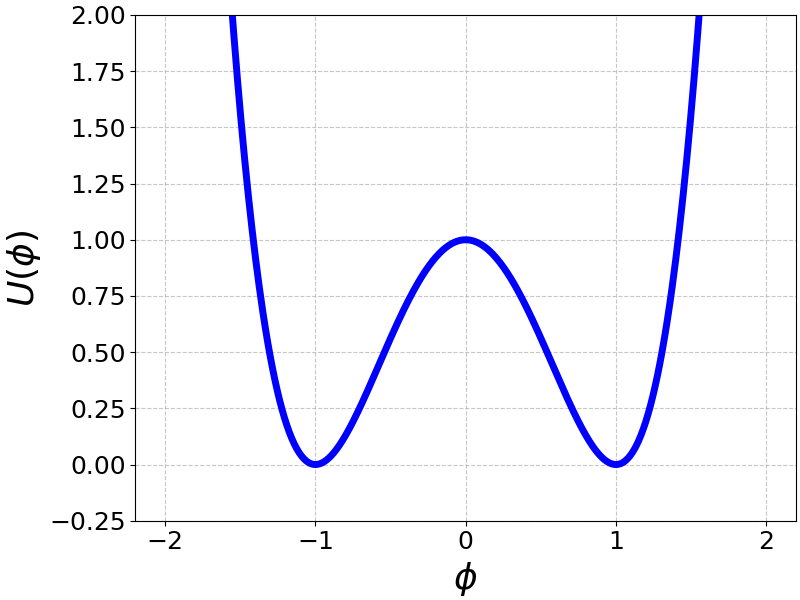
\includegraphics[width=0.6\linewidth]{images/potential.png}
    \caption{Вид потенциала при $\epsilon = 4$.}
    \label{fig:potential}
\end{figure}


%
% difference_scheme.tex
%

\section{Разностная схема}


Уравнения модели фазового поля являются нелинейными уравнениями высокого порядка. В силу этого их теоретический анализ сильно затруднён. Поэтому представляет интерес их численное исследование \cite{elsey_2012, moats_2018, zhuang_2021}


%-------
Для дальнейшего изучения уравнение эволюции фазового поля~($\ref{evolution_eq}$) удобно записать в эквивалентном виде.

Введём поток \(Q\):
\begin{equation*}
    Q \equiv - K \operatorname{grad}\left[\alpha \phi - \beta \Delta \phi + \gamma \Delta^2 \phi +
    \epsilon \phi (\phi^2 - 1)\right].
\end{equation*}

Запишем~($\ref{evolution_eq}$) в виде уравнения непрерывности:
\begin{equation} \label{neprerivn}
    \frac{\partial \phi}{\partial t} + \operatorname{div} (Q) = 0.
\end{equation}

Согласно теореме Остроградского–Гаусса, примененной к области $\omega$ с границей $\partial \omega$, получаем:

\begin{equation*}
    \int \limits_{\omega}  \frac{\partial \phi}{\partial t} \, d V + 
    \oint \limits_{\partial \omega} (Q \cdot dS) = 0.
\end{equation*}
Это соотношение выражает баланс фазового поля $\phi$ в области $\omega$.

В одномерном случае для $\omega = [x_-, x_+]$, имеем:

\begin{equation*}
    \int \limits_{\omega}  \frac{\partial \phi}{\partial t} \, d x + 
    \left [ Q^{+} - Q^{-} \right ] = 0,
\end{equation*}

Откуда:
\begin{equation*}
    0 = \int \limits_{\omega}  \frac{\partial \phi}{\partial t} \, d x + \left [ Q^{+} - Q^{-} \right ] =  | \omega |  \frac{\partial \phi}{\partial t} + \left[ Q^{+} - Q^{-} \right],
\end{equation*}
где $|\omega|$~--- длина интервала, $Q^{-}$ и $Q^{+}$~--- потоки через границы $x_-, x_+$.

%-------


Рассмотрим уравнение на отрезке $\Omega = [0, L] \subset \mathbb{R}$. На границе области будем считать заданными одни из следующих граничных условий:
\begin{enumerate}
    \item периодические граничные условия:
    \begin{equation*}
        \phi(0) = \phi(L), \quad \Delta \phi(0) = \Delta \phi(L), \quad \Delta^2 \phi(0) = \Delta^2 \phi(L);
    \end{equation*}
    \item фиксированные граничные условия:
    \begin{equation*}
        \phi(0) = - \phi(L) = 1, \quad \Delta \phi(0) = \Delta \phi(L) = \Delta^2 \phi(0) = \Delta^2 \phi(L) = 0.
    \end{equation*}
\end{enumerate}
В начальный момент времени при $t = 0$, задано начальное условие 
\begin{equation*}
    \phi(x, 0) = \phi_0(x).
\end{equation*}
Для дискретизации уравнения и граничных условий используем одномерную пространственную сетку с количеством узлов \(N\), шагом \(h\) и временной шаг \( \Delta t \). Пространственные узлы будем нумеровать целыми числами от \(1\) до \(N\).

Первую производную по времени можно аппроксимировать конечной разностью, используя явный метод Эйлера:
\begin{equation*}
    \frac{\partial \phi}{\partial t} \approx \frac{\phi^{n+1}_k - \phi^n_k}{\Delta t},
\end{equation*}
где \( \phi^n_k \) обозначает значение \( \phi \) в точке с индексом \( k \) на временном слое \( n \).

Для лапласиана \( \Delta \phi \) используем центральную разностную схему:

\begin{equation*}
    \Delta \phi_k^n \approx \frac{\phi_{k+1}^n - 2\phi_k^n + \phi_{k-1}^n}{h^2}.
\end{equation*}

Для билапласиана \( \Delta^2 \phi \) используем аналогичную схему:
\begin{equation*}
    \Delta^2 \phi_k^n \approx \frac{\phi_{k+2}^n - 4\phi_{k+1}^n + 6\phi_k^n - 4\phi_{k-1}^n + \phi_{k-2}^n}{h^4}.
\end{equation*}


Теперь мы можем записать выражение для аппроксимации потока \( Q \):
\begin{align*}
    Q_k^n &= K \left(- \alpha \frac{\phi_{k+1}^n - \phi_{k-1}^n}{2h} + \beta \frac{\Delta \phi_{k+1}^n - \Delta \phi_{k-1}^n}{2h} - \right. \\
    &\quad \left. - \gamma \frac{\Delta^2 \phi_{k+1}^n - \Delta^2 \phi_{k-1}^n}{2h} - \epsilon \frac{\phi^{n}_{k+1} \left(  (\phi^{n}_{k+1})^2 - 1 \right) - \phi^{n}_{k-1} \left( (\phi^{n}_{k-1})^2 - 1 \right)}{2h} \right).
\end{align*}

Используя приведённые выше аппроксимации, окончательно получаем дискретное уравнение:
\begin{equation*}
    \phi^{n+1}_k = \phi^n_k - \Delta t \left( \frac{Q_{k+1/2}^n - Q_{k-1/2}^n}{h} \right),
\end{equation*}
где значения потока \( Q \) на границах интервала \( \omega_k \) аппроксимируются как:
\begin{equation*}
    Q_{k+1/2}^n \approx \frac{Q_{k+1}^n + Q_k^n}{2}, \quad Q_{k-1/2}^n \approx \frac{Q_k^n + Q_{k-1}^n}{2}.
\end{equation*}

Поток на границах области $\Omega$ аппроксимируется в соответствии с граничными условиями:
\begin{enumerate}
    \item периодические граничные условия:
    \begin{equation*}
        Q_{1/2}^n \approx \frac{Q_{N}^n + Q_1^n}{2}, \quad Q_{N+1/2}^n \approx \frac{Q_{N}^n + Q_{1}^n}{2};
    \end{equation*}
    \item фиксированные граничные условия:
    \begin{equation*}
        Q_{1/2}^n = 0, \quad Q_{N+1/2}^n = 0.
    \end{equation*}
\end{enumerate}

Свободную энергию системы, соответствующую временному слою $n$, будем аппрокисимировать следующим образом:

\begin{equation*} 
\Psi^n = \sum\limits^{N}_{k=1} \left[ \frac{\alpha}{2}(\phi_k^n)^2 + \frac{\beta}{2}(\nabla \phi_k^n)^2 + \frac{\gamma}{2}(\Delta \phi_k^n)^2 +  \epsilon {\phi_k^n} ({(\phi_k^n)}^2 - 1)) \right] h.
\end{equation*}

Устойчивое численное решение характеризуется монотонным уменьшением свободной энергии системы. В ходе моделирования мы будем строить графики, отображающие изменение свободной энергии в процессе эволюции, чтобы подтвердить корректность численного решения.

Приведённая разностная схема является простейшей явной схемой решения уравнения~({\ref{evolution_eq}}). 
%Она является условно устойчивой с ограничением на шаг по времени \mbox{$\Delta t \sim (\Delta x)^6$}.

%
% simulation_results.tex
%

\section{Результаты моделирования}
%Результаты моделирования-------------------------------------------------------
\subsection{Уравнение Кана-Хилларда}
Рассмотрим упрощённую версию уравнения, положив $\gamma = 0$ для исключения производной высокого порядка, и установим $\epsilon = 1$, $\alpha = 0$. Таким образом, получаем известное уравнение Кана-Хилларда~\cite{cahn_1958}:
\begin{equation*}
    \frac{\partial \phi}{\partial t} = -\operatorname{div}\left\{K \operatorname{grad}\left[\beta \Delta \phi - \phi (\phi^2 - 1)\right]\right\}.
\end{equation*}


Уравнение Кана-Хилларда представляет свой значительный интерес. Оно является базовой математической моделью для описания фазовых переходов в физике твёрдого тела, гидродинамике, задачах солидификации и многих других.
Для этого уравнения известно аналитическое решение:
\begin{equation} \label{analit}
    \phi(x) = \tanh\left(\frac{x} { \sqrt{2  \beta } }\right).
\end{equation}


\begin{figure}[t!]
    \centering
    % First Row
    \begin{minipage}{0.49\linewidth}
        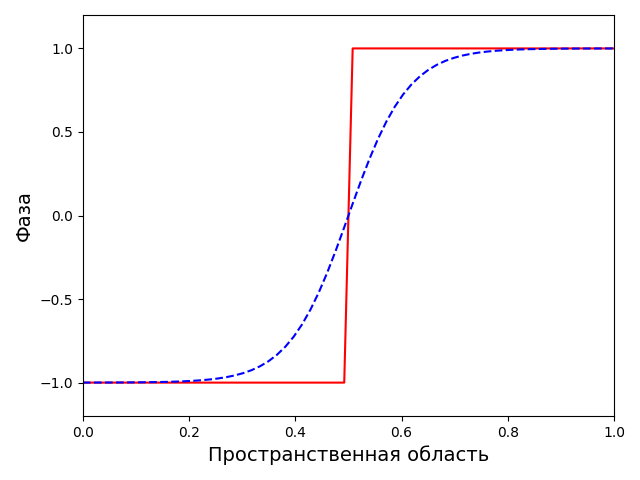
\includegraphics[width=\linewidth]{images/data0.png}
        \subcaption{Фаза при \( t = 0 \): начальное распределение. Сплошная линия~--- численное решение, пунктирная~--- аналитическое решение}
        \label{fig:modeling_KH:1}
    \end{minipage}
    \hfill
    \begin{minipage}{0.49\linewidth}
        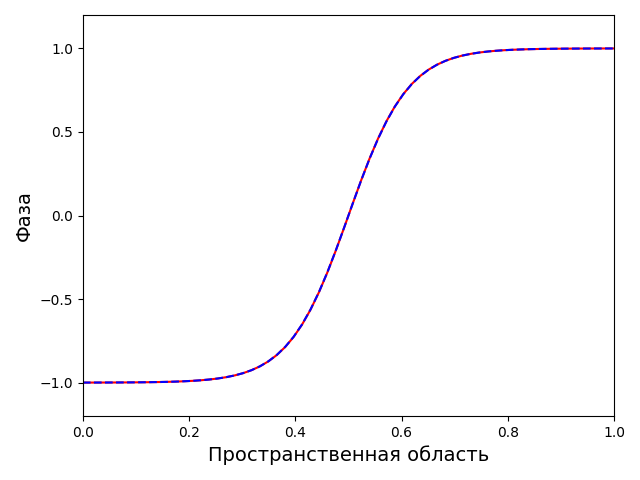
\includegraphics[width=\linewidth]{images/data40000000.png}
        \subcaption{Фаза при \( t = 0.12 \). Сплошная линия~--- численное решение, пунктирная~--- аналитическое решение}
        \label{fig:modeling_KH:2}
    \end{minipage}
    
    % Second Row
    \begin{minipage}{0.49\linewidth}
        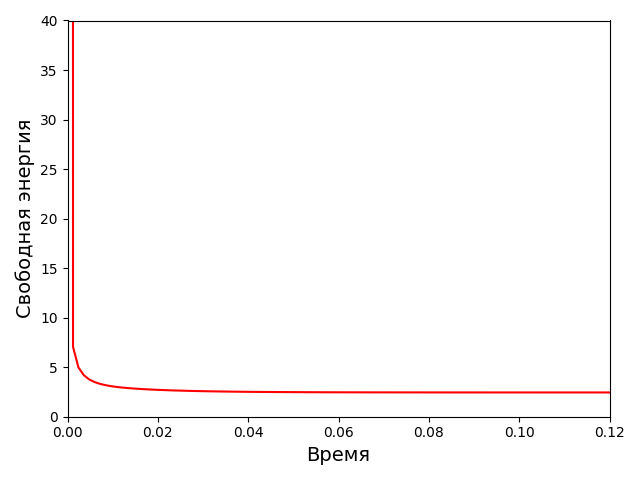
\includegraphics[width=\linewidth]{images/data_energ.png}
        \subcaption{Динамика свободной энергии системы в зависимости от времени \( t \)}
        \label{fig:modeling_KH:3}
    \end{minipage}
    \hfill
    \begin{minipage}{0.49\linewidth}
        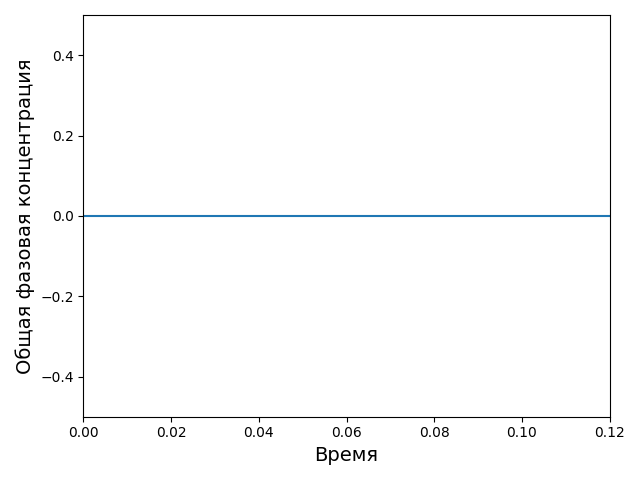
\includegraphics[width=\linewidth]{images/phase_balance.png}
        \subcaption{Сохранение общей концентрации фазы в течении времени \( t \)}
        \label{fig:modeling_KH:4}
    \end{minipage}
    
    \caption{Моделирование уравнения Кана-Хилларда: точное решение и результаты моделирования для различных временных моментов.}
    \label{fig:modeling_KH}
\end{figure}

В экспериментах обычно наблюдается разделение бинарной среды на домены с профилем перехода, который описывается уравнением~(\ref{analit}). Величина $\sqrt{\beta}$ определяет типичную ширину переходного слоя между доменами.
Поскольку для $\phi$ выполняется уравнение непрерывности~(\ref{neprerivn}), в процессе эволюции сохраняется общая концентрация фазы:
\begin{equation*}
    C = \int \limits_{\Omega} \phi(x, t) \, dx, \quad \frac{dC}{dt} = 0.
\end{equation*}
В качестве начального условия моделирования используем две несмешанные фазы, описываемые фазовой функцией:
\begin{equation*}
    \phi(x) = -1.0 + 2.0 \cdot H(x - x_0),
\end{equation*}
где $H(x)$~--- функция Хевисайда.

Для моделирования будем использовать следующие параметры: размер области $L = 1.0$, шаг сетки: $ h = 1 / 64$, временной шаг $\Delta t = h^4 / 20$, параметр $\beta = 25h^2$; подвижность $K = 1$.

Граничные условия задаются как:
\begin{equation*}
\phi(0) = -\phi(L) = -1.0, \nabla^2\phi(0) = \nabla^2\phi(L) = 0.
\end{equation*}

Моделирование показывает, что переходный слой стремится к аналитическому решению~(\ref{analit}) уравнения Кана-Хиларда.
Для подтверждения сохранения концентрации фазы, изобразим динамику баланса фазы во времени на рисунке~\ref{fig:modeling_KH:3}. Кроме того, визуализируем изменение свободной энергии~(\ref{energ}) системы с течением времени на рисунке~\ref{fig:modeling_KH:4}.


\subsection{Одномерный кристалл}
%Одномерный кристалл------------------------------------------------------------
Произведём моделирование кристаллической структуры, эволюция которой описывается уравнением~(\ref{evolution_eq}). В этой модели фазовое поле интерпретируется как атомная плотность.
Зафиксируем параметры уравнения~(\ref{delta psi}) следующим образом: $\beta = -2$, $\gamma = 1$, $\epsilon = 1$, $K = 1$.

Получаем следующее уравнение эволюции:
\begin{equation*}
    \frac{\partial \phi}{\partial t} = \operatorname{div}\left[\operatorname{grad} \left(
    \alpha \phi + 2 \Delta \phi + \Delta^2 \phi +
    \phi^3 - \phi\right)\right].
\end{equation*}

Сделав замену $r = \alpha -2$, приведем это уравнение к виду:

\begin{equation*}
    \frac{\partial \phi}{\partial t} = \frac{\partial \phi}{\partial t} = \Delta\left[
    (1 + \Delta)^2 \phi + \phi^3 + r \phi\right].
\end{equation*}

\label{parametrs1}
Остальные параметры для моделирования положим следующим образом: размер области $L = 40.0$, шаг сетки $\displaystyle h = 0.4$, временной шаг $\displaystyle \Delta t = 10^{-4}$, параметр $r = -0.4$.

Начальное условие выберем как случайное возмущение вблизи нуля со средним значением равным 0, а за граничные условия возьмём периодические граничные условия.

Результаты моделирования показаны на рисунках~\ref{fig:modeling_1_d}. На рисунке~\ref{fig:modeling_1_d:1} показано начальное условие, на рисунках~\ref{fig:modeling_1_d:2}-\ref{fig:modeling_1_d:4}~--- распределение фазового поля в моменты времени $t = 1, 10, 100$. Как видно из полученных графиков, фаза в процессе эволюции принимает вид периодической функции, а свободная энергия монотонно и резко убывает.

\begin{figure}[p]
    \centering
    % First Row
    \begin{minipage}{0.49\linewidth}
        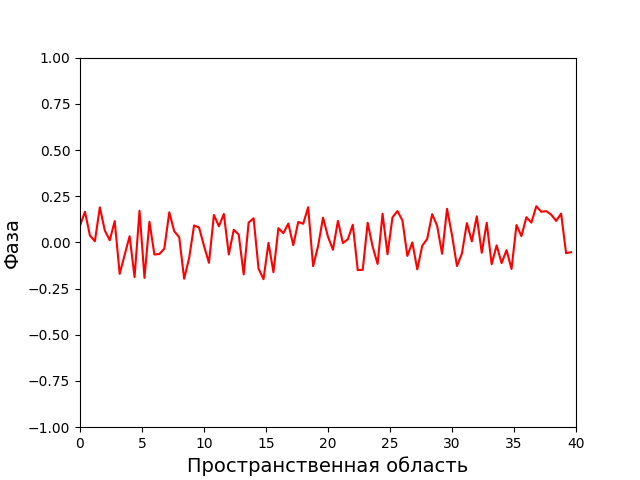
\includegraphics[width=\linewidth]{images/3-data_data_0.bin.png}
        \subcaption{Поле атомной плотности при \( t = 0 \): начальное распределение}
        \label{fig:modeling_1_d:1}
    \end{minipage}
    \hfill
    \begin{minipage}{0.49\linewidth}
        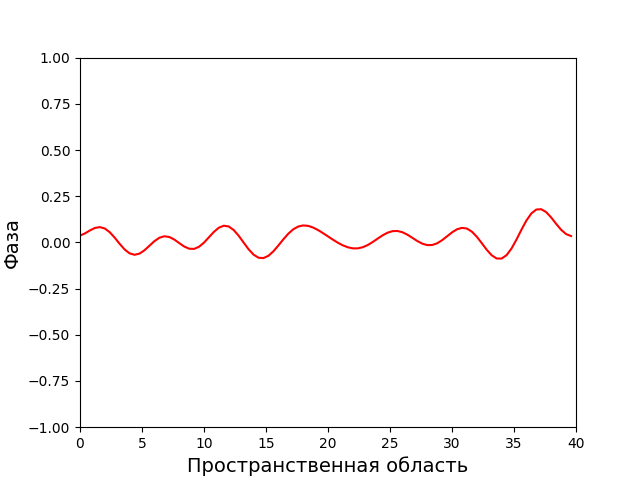
\includegraphics[width=\linewidth]{images/3-data_data_10000.bin.png}
        \subcaption{Поле атомной плотности при \( t = 1 \)}
        \label{fig:modeling_1_d:2}
    \end{minipage}

    % Second Row
    \begin{minipage}{0.49\linewidth}
        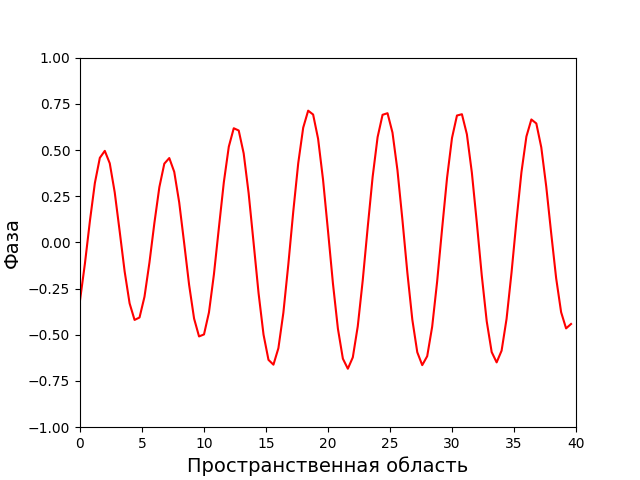
\includegraphics[width=\linewidth]{images/3-data_data_100000.bin.png}
        \subcaption{Поле атомной плотности при \( t = 10 \)}
        \label{fig:modeling_1_d:3}
    \end{minipage}
    \hfill
    \begin{minipage}{0.49\linewidth}
        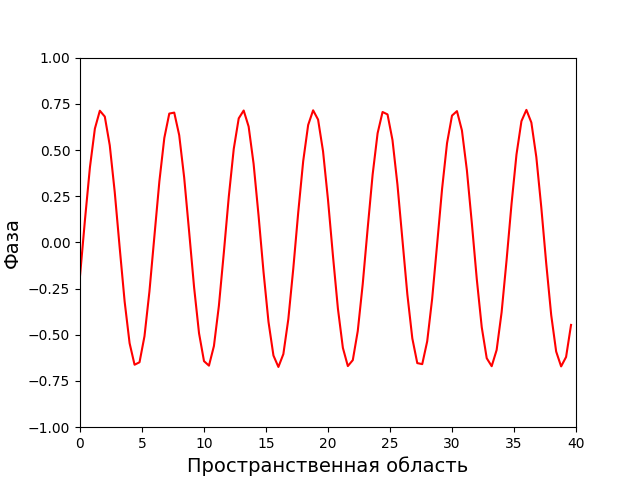
\includegraphics[width=\linewidth]{images/3-data_data_1000000.bin.png}
        \subcaption{Поле атомной плотности при \( t = 100 \)}
        \label{fig:modeling_1_d:4}
    \end{minipage}
    
    % Third Row
    \begin{minipage}{0.49\linewidth}
        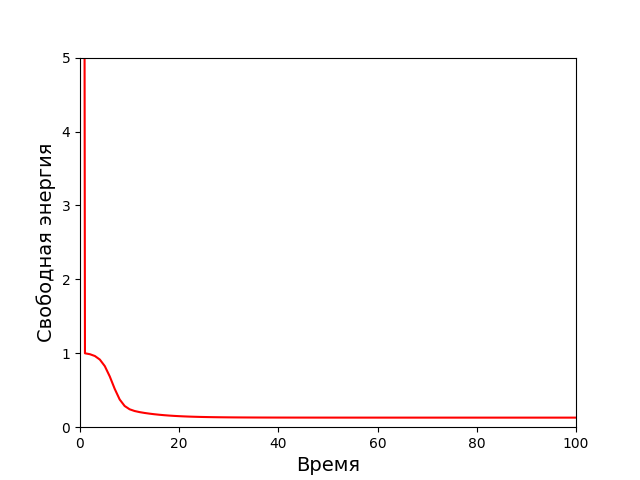
\includegraphics[width=\linewidth]{images/3-energy.png}
        \subcaption{Динамика свободной энергии системы в зависимости от времени \( t \)}
        \label{fig:modeling_1_d:5}
    \end{minipage}
    \hfill
    \begin{minipage}{0.49\linewidth}
        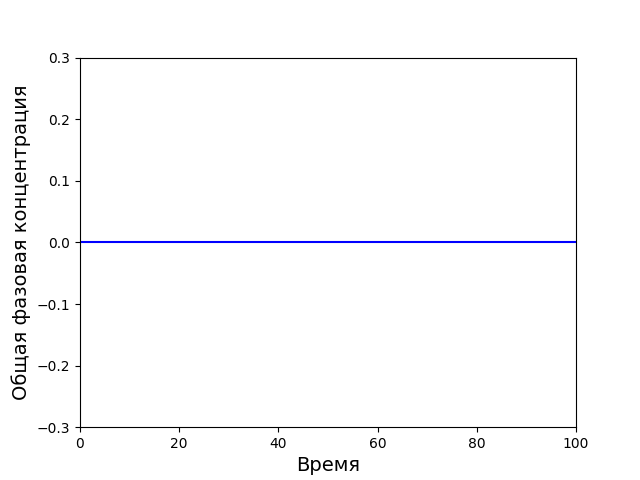
\includegraphics[width=\linewidth]{images/3-phase_balance.png}
        \subcaption{Сохранение общей концентрации фазы в течении времени \( t \)}
        \label{fig:modeling_1_d:6}
    \end{minipage}
    
    \caption{Моделирование одномерной кристаллической структуры}
    \label{fig:modeling_1_d}
\end{figure}


\begin{figure}[p]
    \centering
    % First Row
    \begin{minipage}{0.49\linewidth}
        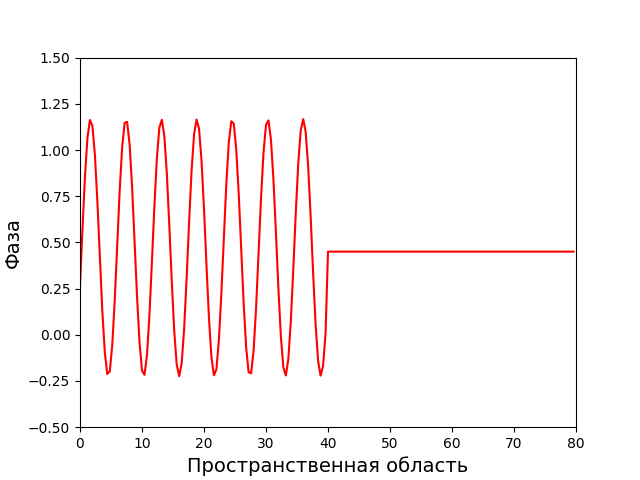
\includegraphics[width=\linewidth]{images/4-data_data_0.bin.png}
        \subcaption{Начальное условие с $\phi_0 = 0.45$}
    \end{minipage}
    \hfill
    \begin{minipage}{0.49\linewidth}
        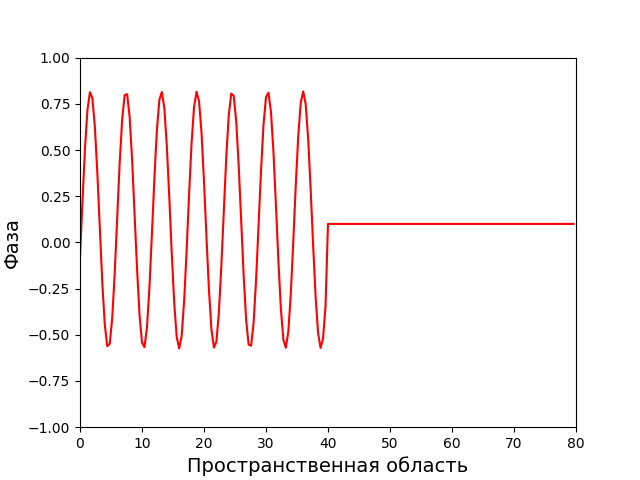
\includegraphics[width=\linewidth]{images/5-data_data_0.bin.png}
        \subcaption{Начальное условие с $\phi_0 = 0.1$}
    \end{minipage}
    \caption{Начальные условия соответствующие двум случаям}
    \label{fig:begin_equation}

    \centering
    % First Row
    \begin{minipage}{0.49\linewidth}
        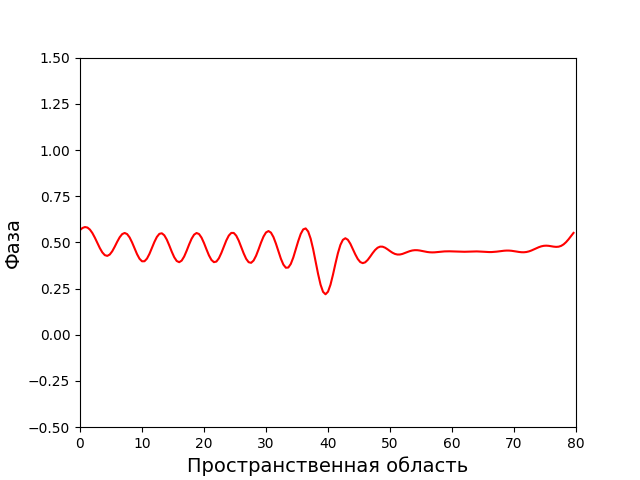
\includegraphics[width=\linewidth]{images/4-data_data_50000.bin.png}
        \subcaption{Фазовое поле при \( t = 5 \)}
    \end{minipage}
    \hfill
    \begin{minipage}{0.49\linewidth}
        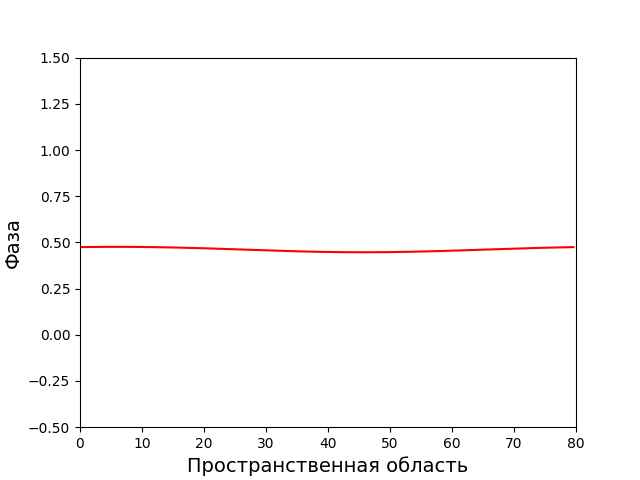
\includegraphics[width=\linewidth]{images/4-data_data_1000000.bin.png}
        \subcaption{Фазовое поле при \( t = 100 \)}
    \end{minipage}
    \caption{Эволюция фазовой функции в первом случае}
    \label{fig:evolution_1}

    \centering
    % First Row
    \begin{minipage}{0.49\linewidth}
        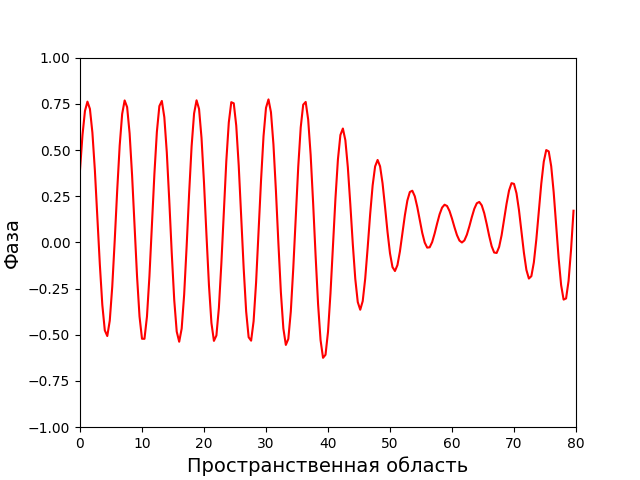
\includegraphics[width=\linewidth]{images/5-data_data_50000.bin.png}
        \subcaption{Фазовое поле при \( t = 5 \)}
    \end{minipage}
    \hfill
    \begin{minipage}{0.49\linewidth}
        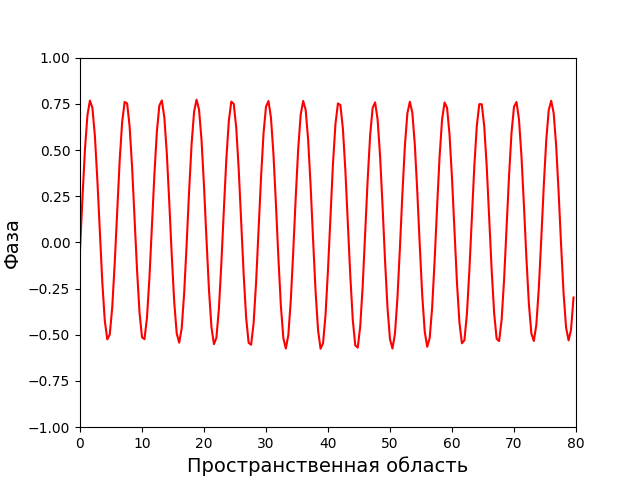
\includegraphics[width=\linewidth]{images/5-data_data_1000000.bin.png}
        \subcaption{Фазовое поле при \( t = 100 \)}
    \end{minipage}
    \caption{Эволюция фазовой функции во втором случае}
    \label{fig:evolution_2}
\end{figure}

\subsection{Зависимость амплитуды фазового поля\\от параметров}
Параметр $r$ играет роль температуры. 
\begin{equation*}
    r \sim \frac{T - T_c}{T_c},
\end{equation*}
где $T_c$~--- температура кристаллизации.

В статье Элдера и Гранта~\cite{elder_2004} анализируется зависимость амплитуды фазовой функции, получающейся в процессе эволюции, от параметра $r$ и начального распределения фазы. Приводится следующее выражение:
\begin{equation*}
    A = 2 \sqrt{- r / 3 - \phi_0^2},
\end{equation*}
где $A$~--- амплитуда фазовой функции, а $\phi_0$~--- среднее значение фазы.
В случае отрицательного значения выражения под корнем, фаза в процессе эволюции стремится к константе, что соответствует распределению фазы в жидкости.

Таким образом, даже при температуре меньшей температуры кристаллизации и отрицательном параметре $r$ кристаллизации может не происходить по причине достаточно большой средней фазовой концентрации $\phi_0$.

Смоделируем два случая соответствующие разным знакам выражения под корнем за счёт изменения среднего значения фазы. Моделирование будем проводить на области размером $2 L = 80.0$, a начальное условие будем задавать в виде:
\[
\phi(x) = 
\left\{
\begin{array}{ll}
    \phi_0 + \phi^*(x), & 0 \leqslant x < L,\\
    \phi_0, & L \leqslant x < 2 L,
\end{array}
\right.
\]
где $\phi^*(x)$~--- фазовая функция получаемая в результате моделирования с параметрами из раздела~(\ref{parametrs1}). Среднее значение будет принимать значения $0.45$ в первом случае и $0.1$ во втором. Остальные параметры положим как в разделе~(\ref{parametrs1}).

На рисунках~\ref{fig:begin_equation} приведены графики начального распределения фазы в обоих случаях, отличающихся друг от друга средним значением фазы. Они могут быть интерпретированы как кристалл помещённый в жидкость при температуре и фазовой концентрации соответствующих плавлению кристалла в первом случае и кристаллизации жидкости во втором.

Рисунки~\ref{fig:evolution_1} соответствуют эволюции фазовой функции в случае большего значения фазы. В процессе эволюции наблюдается плавление кристалла. Получаемое в результате $100$ секунд эволюции распределение близко к константе и имеет физический смысл распределения атомной плотности в жидкости.

Рисунки~\ref{fig:evolution_2} соответствуют эволюции фазовой функции в случае меньшего среднего значения фазы. В процессе эволюции наблюдается кристаллизация жидкости. Получаемое в результате $100$ секунд эволюции распределение отлично от константы и имеет периодическую структуру. Физический смысл получающегося распределения фазы~--- атомная плотность в кристалле.


%
% conclusion.tex
%

\section{Заключение}

В работе был проведён анализ метода фазового поля в контексте моделирования бинарной среды и кристаллических структур.

Было выполнено численное моделирование уравнения Кана-Хилларда. Результаты этого моделирования были сопоставлены с аналитическим решением. Было продемонстрировано соответствие получаемого в процессе эволюции раздела между двумя средами аналитическому решению.

Кроме того, было проведено моделирование кристаллической структуры, где полученное периодическое распределение фазы соответствует периодическому распределению атомов в кристаллической решетке.

В рамках исследования был осуществлен анализ влияния параметров модели и начальных условий на процесс формирования кристаллической структуры. Проведено моделирование, соответствующее двум различным результатам временной эволюции: постоянному распределению фазы и периодическому.



\clearpage
%
% references.tex
%

\begin{thebibliography}{99}

  % %%% C %%%%%%%%%%%%%%%%%%%%%%%%%%%%%%%%%%%%%%%%%%%%%%%%%%%%%%%%%%%%%%%%%%%%%%
\bibitem[Chen2002]{chen_2002}
  Chen, L. Q.
  Phase-field models for microstructure evolution //
  Annual Review of Materials Research, vol.~32, 2002, pp.~113–140.
  \url{https://doi.org/10.1146/annurev.matsci.32.112001.132041}

\bibitem[Cahn1958]{cahn_1958}
    Cahn, J. W.; Hilliard, J. E.
    Free Energy of a Nonuniform System. I. Interfacial Free Energy //
    The Journal of Chemical Physics, vol.~28, no.~2, February 1958, pp.~258–267.
    \url{https://doi.org/10.1063/1.1744102}

  % %%% E %%%%%%%%%%%%%%%%%%%%%%%%%%%%%%%%%%%%%%%%%%%%%%%%%%%%%%%%%%%%%%%%%%%%%%
\bibitem[Elder2002]{elder_2002}
  Elder, K. R., Katakowski, M., Haataja, M., Grant, M.
  Modeling Elasticity in Crystal Growth //
  Physical Review Letters, vol.~88, no.~24, June 17, 2002.
  \url{https://doi.org/10.1103/PhysRevLett.88.245701}

\bibitem[Elder2004]{elder_2004}
  Elder, K. R., Grant, M.
  Modeling elastic and plastic deformations in nonequilibrium processing using phase field crystals //
  Physical Review E, vol.~70, 051605, November 19, 2004.
  \url{https://doi.org/10.1103/PhysRevE.70.051605}

\bibitem[Elsey2012]{elsey_2012}
  Elsey, M., Wirth, B.
  A simple and efficient scheme for phase field crystal simulation //
  Journal of Computational Physics, vol.~231, no.~9, April 2012, pp.~3645–3663.
  \url{https://doi.org/10.1051/m2an/2013074}

  % %%% M %%%%%%%%%%%%%%%%%%%%%%%%%%%%%%%%%%%%%%%%%%%%%%%%%%%%%%%%%%%%%%%%%%%%%%
\bibitem[Moats2018]{moats_2018}
  Moats, K. A.
  The Development of a Numerical Solver for the Phase Field Crystal Model with Select Applications to Materials Science //
  University of Memphis Digital Commons, Electronic Theses and Dissertations, April 19, 2018.

  % %%% Z %%%%%%%%%%%%%%%%%%%%%%%%%%%%%%%%%%%%%%%%%%%%%%%%%%%%%%%%%%%%%%%%%%%%%%
\bibitem[Zhuang2021]{zhuang_2021}
  Zhuang, Debbie
  A 1-D Phase Field Crystal Model for Li-ion Battery Intercalation with Lattice Volume Changes //
  Department of Chemical Engineering, Massachusetts Institute of Technology, May 21, 2021.

\end{thebibliography}


% %%%%%%%%%%%%%%%%%%%%%%%%%%%%%%%%%%%%%%%%%%%%%%%%%%%%%%%%%%%%%%%%%%%%%%%%%%%%%%

\clearpage
\tableofcontents

\end{document}

% EOF

